\documentclass[a4paper,10pt]{article}

\usepackage[utf8]{inputenc}
\usepackage[english]{babel}
\usepackage[T1]{fontenc}
\usepackage{mathpazo} %http://www.ctan.org/tex-archive/fonts/mathpazo
\usepackage{stmaryrd} %http://www.ctan.org/pkg/stmaryrd
\usepackage{amsmath} %http://www.ctan.org/pkg/amsmath
\usepackage{amssymb}
\usepackage{mathrsfs}
\usepackage{subfig}

\usepackage{cite}

\usepackage{amsthm} %http://www.ctan.org/pkg/amsthm
\usepackage{proof}
\usepackage{algorithm2e}

\usepackage[colorlinks=true]{hyperref} %http://www.ctan.org/tex-archive/macros/latex/contrib/hyperref/
\hypersetup{urlcolor=black,linkcolor=black}
\usepackage{footmisc} %http://www.ctan.org/tex-archive/macros/latex/contrib/footmisc

\usepackage{enumerate}
\usepackage{ulem} %http://www.ctan.org/tex-archive/macros/latex/contrib/ulem
\normalem
\usepackage{cancel} %http://www.ctan.org/tex-archive/macros/latex/contrib/cancel

\usepackage{fullpage} %http://www.ctan.org/tex-archive/macros/latex/contrib/preprint/
\setlength{\parindent}{0pt}
\setlength{\parskip}{\medskipamount}

\usepackage{pgffor}
\usepackage{tikz}
\usetikzlibrary{arrows,shapes.arrows, chains, positioning, automata, graphs, decorations.pathreplacing}

%\usepackage[ruled,vlined,french]{algorithm2e}
%\providecommand{\SetAlgoLined}{\SetLine}
%\providecommand{\DontPrintSemicolon}{\dontprintsemicolon}

%\usepackage{forest}
\usepackage{comment} %http://www.ctan.org/tex-archive/macros/latex/contrib/comment
\usepackage{multirow} %http://www.ctan.org/tex-archive/macros/latex/contrib/multirow
\usepackage{diagbox} %http://www.ctan.org/tex-archive/macros/latex/contrib/diagbox

\usepackage{textcomp} %http://www.ctan.org/pkg/textcomp

\usepackage{listings} %http://www.ctan.org/tex-archive/macros/latex/contrib/listings/
\lstset{numbers=left,language=Caml}

\usepackage{boiboites}
\newboxedtheorem[boxcolor=orange, background=blue!5, titlebackground=blue!20,
titleboxcolor = black]{theo}{Theorem}{compteurTh}
\newboxedtheorem[boxcolor=orange, background=blue!5, titlebackground=blue!20,
titleboxcolor = black]{defi}{Definition}{compteurDef}

\newcounter{ThComp}
\newcounter{DefComp}

\newboxedtheorem[boxcolor=red, background=red!5, titlebackground=red!50,titleboxcolor = black]{theoreme}{Th\'{e}or\`{e}me}{TheC}
\newboxedtheorem[boxcolor=orange, background=orange!5, titlebackground=orange!50,titleboxcolor = black]{definition}{D\'{e}finition}{DefC}
\newboxedtheorem[boxcolor=blue, background=blue!5, titlebackground=blue!20,titleboxcolor = black]{proposition}{Proposition}{ProC}
\newboxedtheorem[boxcolor=cyan, background=cyan!5, titlebackground=cyan!20,titleboxcolor = black]{corollaire}{Corollaire}{CorC}
\newboxedtheorem[boxcolor=black, background=black!0, titlebackground=black!20,titleboxcolor = black]{remarque}{Remarque}{RemC}
\newboxedtheorem[boxcolor=green!70!black, background=green!70!black!5, titlebackground=green!70!black!30,titleboxcolor = black]{notation}{Notation}{NotC}
\newboxedtheorem[boxcolor=yellow, background=yellow!0, titlebackground=yellow!30,titleboxcolor = black]{exemple}{Exemple}{ExeC}
\newboxedtheorem[boxcolor=magenta, background=magenta!5, titlebackground=magenta!30,titleboxcolor = black]{lemme}{Lemme}{LemC}

\newcommand{\ra}{\rightarrow}
\newcommand{\la}{\leftarrow}


\newcommand{\RR}{\mathbb{R}}
\newcommand{\ZZ}{\mathbb{Z}}
\newcommand{\Ztwo}{\mathbb{Z}^{2}}
\newcommand{\NN}{\mathbb{N}}
\newcommand{\PP}{\mathbb{P}}
\newcommand{\EE}{\mathbb{E}}
\newcommand{\IE}{\mathbb{E}}
\newcommand{\IR}{\mathbb{R}}
\newcommand{\IZ}{\mathbb{Z}}
\newcommand{\IN}{\mathbb{N}}
\newcommand{\IP}{\mathbb{P}}

\newcommand{\cF}{\mathcal{F}}
\newcommand{\ck}{\mathcal{K}}
\newcommand{\cL}{\mathcal{L}}
\newcommand{\cN}{\mathcal{N}}
\newcommand{\cNU}{\mathcal{NU}}
\newcommand{\A}{\mathcal{A}}
\newcommand{\B}{\mathcal{B}}
\newcommand{\F}{\mathcal{F}}
\renewcommand{\L}{\mathcal{L}}
\newcommand{\N}{\mathcal{N}}

\newcommand{\ens}[1]{\left\{ #1 \right\}}
\newcommand{\set}[1]{\left\{ #1 \right\}}
\renewcommand{\leq}{\leqslant}
\renewcommand{\geq}{\geqslant}
\renewcommand{\le}{\leqslant}
\renewcommand{\ge}{\geqslant}
\newcommand{\cplx}[1]{\mathcal O \left( #1 \right)}
\newcommand{\floor}[1]{\left \lfloor #1 \right \rfloor}
\newcommand{\ceil}[1]{\left\lceil #1 \right\rceil}
\newcommand{\brackets}[1]{\left\llbracket #1 \right\rrbracket}
\newcommand{\donne}{\rightarrow}
\newcommand{\gives}{\rightarrow}
\newcommand{\dans}{\to}
\newcommand{\booleen}{\set{0,1}^*}
\newcommand{\eps}{\varepsilon}
\renewcommand{\implies}{~\Rightarrow~}
\newcommand{\tildarrow}{\rightsquigarrow}
\newcommand{\blank}{\texttt{\char32}}
\newcommand{\trans}[1]{\xrightarrow{#1}}
\newcommand{\rules}[1]{\xrightarrow{#1}}
\newcommand{\todo}[1]{\Large\textcolor{red}{#1}\normalsize}
\newcommand{\argmin}{\text{argmin}}
\newcommand{\rainbowdash}{\vdash}
\newcommand{\notrainbowdash}{\nvdash}
\newcommand{\rainbowDash}{\vDash}
\newcommand{\notrainbowDash}{\nvDash}
\newcommand{\Rainbowdash}{\Vdash}
\newcommand{\notRainbowdash}{\nVdash}
\newcommand{\bottom}{\bot}

%TD/TP
\newenvironment{answer}{\color{blue}}{}


%EvalPerf
\newcommand{\Var}{\text{Var}}
\newcommand{\prob}[1]{\PP\left( #1 \right)}
\newcommand{\esp}[1]{\EE\left( #1 \right)}


%SystDist
\newcommand{\Receive}{\texttt{Receive~}}
\newcommand{\Send}{\texttt{Send~}}


%Preuves
\newcommand{\betaeq}{=_\beta}
\newcommand{\betared}{\vartriangleright_\beta}
\newcommand{\parabetared}{\vartriangleright_{||\beta}}
\newcommand{\Ackermann}{\A}


%Cplx
\newcommand{\Time}{\textsc{Time}}
\newcommand{\TIME}{\textsc{Time}}

\newcommand{\dtime}{\textsc{DTime}}
\newcommand{\dTime}{\textsc{DTime}}
\newcommand{\DTime}{\textsc{DTime}}

\newcommand{\ntime}{\textsc{NTime}}
\newcommand{\nTime}{\textsc{NTime}}
\newcommand{\NTime}{\textsc{NTime}}

\renewcommand{\P}{\textsc{P}}

\newcommand{\pTime}{\textsc{PTime}}
\newcommand{\PTime}{\textsc{PTime}}

\newcommand{\NP}{\textsc{NP}}

\newcommand{\npTime}{\textsc{NPTime}}
\newcommand{\NPTime}{\textsc{NPTime}}

\newcommand{\EXP}{\textsc{Exp}}
\newcommand{\expTime}{\textsc{Exp}}
\newcommand{\ExpTime}{\textsc{Exp}}
\newcommand{\EXPTime}{\textsc{Exp}}

\newcommand{\Space}{\textsc{Space}}

\newcommand{\dSpace}{\textsc{DSpace}}
\newcommand{\DSpace}{\textsc{DSpace}}


\newcommand{\nSpace}{\textsc{NSpace}}\newcommand{\NSpace}{\textsc{NSpace}}

\newcommand{\pSpace}{\textsc{PSpace}}
\newcommand{\PSpace}{\textsc{PSpace}}

\newcommand{\npSpace}{\textsc{NPSpace}}
\newcommand{\NpSpace}{\textsc{NPSpace}}
\newcommand{\NPSpace}{\textsc{NPSpace}}

\newcommand{\SpaceTM}{\textsc{SpaceTM}}

\newcommand{\nL}{\textsc{NL}}
\newcommand{\NL}{\textsc{NL}}

\newcommand{\LL}{\textsc{L}}

\newcommand{\coNP}{co\text{-}\textsc{NP}}

\newcommand{\conL}{co\text{-}\textsc{NL}}
\newcommand{\coNL}{co\text{-}\textsc{NL}}

\newcommand{\npc}{\text{\textit{NP-C}}}

\newcommand{\PH}{\textsc{PH}}

\newcommand{\TISP}{\textsc{TISP}}

\newcommand{\Size}{\textsc{Size}}
\newcommand{\SIZE}{\textsc{Size}}





\title{A binary shape indexing/retrieval system}
\author{
    William \textsc{Aufort}\\
    Marc \textsc{Chevalier}
}
\date{\today}

\begin{document}
\maketitle

\section*{Introduction}

\subsection*{General introduction}

The objective of this project is to design a binary shape indexing system. Given a database of binary shapes (PGM files) associated to different classes, and a binary image, the goal is to find the class which correspond the most to the image.
One important problem of image classification based is the definition of a suitable metric to measure similarity between two images. In this document, we present and explain our main ideas to solve the problem and our implementation choices.

\subsection*{The database used}

In this project, we have access to a database of about 1000 images in the PGM format. All these images are made with two gray levels, respectively black and white. Excepted for one image (\texttt{rat-09.pgm}\footnote{We can't really explain why, but that's it...}), the object is defined by the white component. The database contains 70 classes, that we can divide into three main categories:
\begin{itemize}
	\item the objects (vehicles, usual objects like phones, watches, ...);
	\item the animals (for instance, camels, octopuses, children, ...);
	\item and the geometric shapes (most of them denoted by \texttt{device-i} for some $i$).
\end{itemize}

The figure \ref{shapedata} illustrates these three categories.

Of course, other decompositions, more or less precise, are possible. From this, we just have to keep in mind that such a diversity on the objects to study is a real difficulty to algorithm design.

\begin{figure}[!ht]
    \centering
    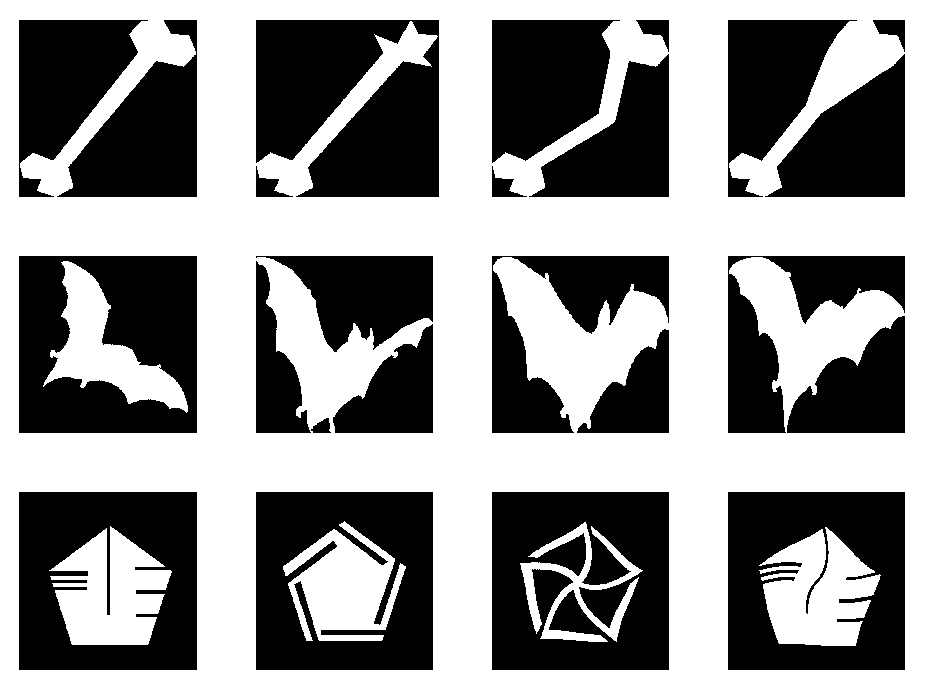
\includegraphics[height=175pt]{../database/shapedata.eps}
	\caption{A panel of objects of the database: bats, bones and geometrical objects}
	\label{shapedata}
\end{figure}


\section{How to deal with noise: choices and implementation}

First of all, an important aspect of the project is to deal with image which can be potentially noised.

More precisely, we were interested in deleting specular noise. In particular, the \textsc{Kanungo} noise used in the evaluation of our method is a kind of specular noise, because it's a local swapping procedure. Our choice is to implement a binomial filter saw during the course. This filter, used essentially for smoothing grayscale images, erases the potential specular noise on the image. If the image is not noisy, the experiment show that the initial image is not modified. The initial filter (i.e. for a grayscale image) is:

\setcounter{MaxMatrixCols}{3}
\[ F = \quad \frac{1}{16} \begin{pmatrix}
1 & 2 & 1 \\
2 & 4 & 2 \\
1 & 2 & 1
\end{pmatrix}\]

In the grayscale output image, we only keep the pixels with intensity greater than $8 \times 255$, where $8$ represents half of the sum of the weights in the filter ($16$ here) and $255$ the intensity for the white part of the image (i.e. the final object we keep). For more simplicity, we don't keep the $255$ factor, since the only possible intensity values in the input image are $0$ and $255$.

We give a simpler implementation of the filter. One could improve it, for example using the fact that this filter is separable to decompose the calculations into two less costly steps.

\section{Granulometric analysis}

\subsection{Basic ideas}

When we are watching images, to associate them to concepts, we use our knowledge of these concepts. For example, an apple is a quite circular object with sometimes a stalk and leaves, a camel is a mammal with one or two humps, etc.. Basically, for organic objects, we use a kind of segmentation characterisation to identify the concepts: we recover it by identify its different parts.

A famous tool used in volumetric analysis to determine segmentation is the \textbf{granulometric function}. Indeed, it plays an important role for shape description, what we want exactly to do.

\begin{definition}[Granulometric function]
Let $\mathcal{X}$ be a binary shape in $\Ztwo$. We denoted by $B(c,r)$ the euclidean ball with center $c \in \Ztwo$ and radius $r \in \RR$. We define the granulometric function $g_{\mathcal{X}}$ on $\mathcal{X}$ by:

$$ g_{\mathcal{X}}(x) = \operatorname{max} \left\{ r | \exists c \in \mathcal{X}, x \in B(c,r) \wedge B(c,r) \subseteq \mathcal{X} \right\} $$ 
\end{definition}

In other words, we are looking for the radius of the greatest ball included in the shape $\mathcal{X}$ which contains our point $x$.

If we plot the granulometry function on a 2D shape in the database, we can observe that the different values of the granulometric function correspond to the different "parts" of the object. An example is given on figure \ref{apple-granulo}.

\begin{figure}[!ht]
    \centering
    \subfloat{
        \label{apple-granulo:1}   
        
\includegraphics[height=175pt]{images/apple-1}
    }
    \qquad\qquad\qquad
    \subfloat{
        \label{apple-granulo:2}
        \includegraphics[height=175pt]{images/apple-1-granulo}
    }
    \caption{The granulometric function illustrated in this apple image. We can easily distinguish the different natural parts of the apple using the granulometric function.}
    \label{apple-granulo}
\end{figure}

We can use the granulometric function to compare two images. To do this, we can see the granulometric function as a distribution of the radius of the maximal balls over the object $\mathcal{X}$, which can be describes for examples with histograms like those we use in statistics.

% TODO: Histograms construction

Compare two images remains to compare two histograms, so we have to define a distance between histograms. This work will be explained with more details in the next section.

\subsection{Advantages}

\subsubsection{Invariant by translation, rotation, scaling and symmetry}

The invariance with respect to translation, rotation and symmetry is an important property. But we have to be a little bit more precise:

\begin{theoreme}[Invariance by translation]
	Let $\mathcal{X}$ be a binary shape in $\Ztwo$. Let $\vec{t} \in \Ztwo$ be a vector of translation, and let $\mathcal{X}_{t} = \left\{ x + \vec{t}, x \in \mathcal{X} \right\}$. Then:
	
	$$ \forall x \in \mathcal{X}_{t}, g_{\mathcal{X}_{t}}(x) = g_{\mathcal{X}}(x-\vec{t}) $$
\end{theoreme}

In other words, there is a trivial isomorphism between the two images $\mathcal{X}$ and  $\mathcal{X}_t$ seen as unions of balls. With this remark, the proof of the theorem is completely trivial.

But the same result for rotations is not completely trivial. If we take a rotation of any angle, one can imagine that the pixels of the image, after the rotation, don't match exactly with points in $\Ztwo$, because of the trigonometric functions implied during the process. The same behaviour occurs if we consider symmetries with respect to any line or center, a translation of a vector $v \in \RR^2$, or a scaling with any scaling factor.


What's more, all these properties holds for the continuous version of the granulometric function (i.e. where $\mathcal{X}$ is a shape in $\RR^2$). Indeed, we clearly have:

\begin{remarque}[Properties for $\mathcal{X} \subset \RR^2$]
	\begin{itemize}
		\item If $t : \RR^2 \to \RR^2$ is a translation, then $\forall x \in \mathcal{X}, g_{t(\mathcal{X})}(x) = g_{\mathcal{X}}(t^{-1}(x))$, where $t^{-1}$ is the translation of vector $-\vec{t}$.
		\item If $r : \RR^2 \to \RR^2$ is a rotation of center $c$ and angle $\theta$, then $\forall x \in \mathcal{X}, g_{r(\mathcal{X})}(x) = g_{\mathcal{X}}(r^{-1}(x))$, where $r^{-1}$ is the rotation of center $c$ and angle $-\theta$. 
		\item If $h : \RR^2 \to \RR^2$ is an homothetic transformation of center $c$ and ration $\lambda$, then $\forall x \in \mathcal{X}, g_{h(\mathcal{X})}(x) = \lambda \times g_{\mathcal{X}}(h^{-1}(x))$, where $h^{-1}$ is the homothetic transformation of center $c$ and ratio $\frac{1}{\lambda}$.
	\end{itemize}
\end{remarque}

% TODO Check all these theorems

The proof works as the previous one, with writing the isomorphisms between the two images.

Hence nonetheless, intuitively if there exists some modifications in the granulometric function, they are not going to be very large, but it's difficult to quantify this difference.

\subsection{Disadvantages}

\subsubsection{Geometrical objects with perturbations}

Some of the classes are defined by the basic geometrical object they refers to. For example, the object presented in the figure \ref{device9-6}, as all the elements in the class \texttt{device9}, are very close to a ball, excepted that they are crossed by some perturbing element (in the figure it's a line). The problem on such images is that that king of noise perturb a lot the output of the granulometric function, as we can see in the figure \ref{device9-6}.

\begin{figure}[!ht]
    \centering
    \subfloat{
        \label{device9-6:1}
        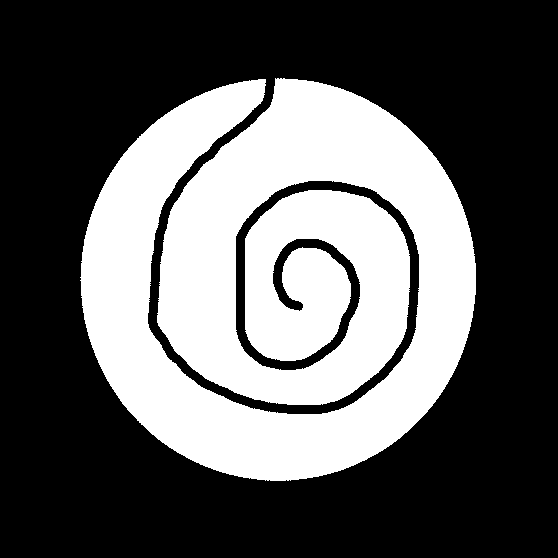
\includegraphics[height=175pt]{images/device9-6-object}
    }
    \qquad\qquad\qquad
    \subfloat{
        \label{device9-6:2}
        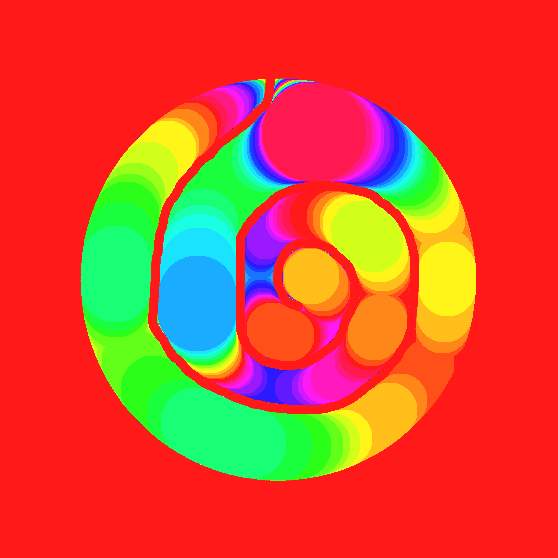
\includegraphics[height=175pt]{images/device9-6-granulo}
    }
    \caption{The granulometric function is very perturbed on this geometrical object crossed by a curve.}
	\label{device9-6}
\end{figure}

\subsubsection{Loss of spatial information}

One of the problem of this method is to not take into account the distribution of the values on the image, or in the space more generally. For example, you cannot distinguish between a disk and a donut or a rope only with the granulometric function, because for all these objects, the function is constant. Some methods use a decomposition of the image into different regions and then divides the computations spatially, for example \cite{spacial-decompo}, and it could be interesting to adapt such methods with the granulometric function.

\subsubsection{Robustness in presence of (specular) noise}

As we can guess, the balls of the initial image won't be available for the noisy image. There must be more balls with small radius, which clearly perturb the granulometric function. That's why we need a noise filter as the one we exposed in the first 

\subsubsection{Computation time}

As we will see in the further section, the time needed to compute this function is quite important, and it's really a mess to evaluate it on all the images of the database. Indeed, for one image, the execution time can exceed two hours, which is unusable in practice.

\subsection{Implementation}

The general idea of the algorithms that computes the granulometric function is to get a quite good set of candidate balls. A ball included in the image is a candidate ball if it must have a contribution on the granulometric function of a point of the image. Indeed, most of the complexity of the algorithm leads on the iterator over those balls in order to compute the maximal radius for each point. 

We present two algorithms. The first one is quite naive and have been implemented first. It uses only the distance transformation (DT). The second one, closer to the medial axis concept, is an optimization where we drastically reduce the number of candidate balls to scan.

\subsubsection{Naive algorithm: Distance Transformation}

We recall the definition of the Distance Transformation saw during the class:

\begin{definition}[Distance transformation]
Let $\mathcal{X}$ be a binary shape in $\Ztwo$. If $p$ is a point of $\mathcal{X}$, we called the Distance transformation at $p$, denoted by $DT(p)$, the smallest distance to the border of the image:
$$ DT(p) = \underset{q \in \widetilde{\mathcal{X}}}{min} \quad d(p,q) $$
\end{definition}

$DT(p)$ represents the maximum radius of a ball containing $p$, included in $\mathcal{X}$. We are interested in it because of this trivial result:

\begin{theoreme}
	For all $p \in \mathcal{X}$, for all $r$ such that $B(p,r) \subset \mathcal{X}$, we have:
		$$ B(p,r) \subset B(p,DT(p))$$
\label{theoremDT}
\end{theoreme}

With this result, we can restrict the number of balls to scan to $\cplx{\left| \mathcal{X} \right|}$. Indeed, we can consider only the balls $\set{B(p,DT(p)), p \in \mathcal{X}}$, because of the other balls are included in some of those ones.

\begin{proof}
	
Let us suppose that $B(p,r) \nsubseteq B(p,DT(p))$ for some $p$ and $r$. This implies that $r > DT(p)$.

Let $p'$ be the point of the border $\widetilde{\mathcal{X}}$ such that $d(p,p') = DT(p)$. Let $q = p + (p'-p).\frac{r}{DT(p)}.$ 

$d(p,q) = \frac{r}{DT(p)}.d(p,p') = r > DT(p)$. Hence, by construction of $q$, we can deduce that $q \notin \mathcal{X}$, so we get a contraction with $q \in B(p,r) \subset \mathcal{X}$. 

\end{proof}

We use the implementation of the Distance Transformation provided in \textsc{DGtal}. Once we have computed the Distance Transformation, the naive algorithm we can use to compute the granulometric function works as follows:

\IncMargin{1em}
\begin{algorithm}
\ForEach{point $p \in \mathcal{X}$}{
    Create a ball centered at $p$ with radius $DT(p)$\;
    \ForEach{point $q$ in this ball}{
        \If{$g(y) \leq DT(p)$}{
			$g(y) \leftarrow DT(p)$\;
		}
	}
}
\caption{Naive algorithm to compute the granulometric function $g$}
\label{algo-naive}
\end{algorithm}

\begin{theoreme}[Correctness of Algorithm \ref{algo-naive}]
	At the end of the execution of the algorithm \ref{algo-naive}, $g$ is exactly the granulometry function on $\mathcal{X}$.
\end{theoreme}

\begin{proof}
Let $p \in \mathcal{X}$. We can easily see that the value returned for $g(p)$ at the end of the algorithm is 
$ \operatorname{max} \set{DT(q) | q \in \mathcal{X} \wedge p \in B(q,DT(q)) \subset \mathcal{X}} 
= \operatorname{max} \set{r | q \in \mathcal{X} \wedge p \in B(q,r) \subset \mathcal{X}}$ thanks to Theorem \ref{theoremDT}, which is exactly $g(p)$.
\end{proof}

The complexity of this algorithm is quite bad. For each point $p$, we build a ball of radius $DT(p)$ and scan all the points inside the ball to (eventually) update some values of granulometry. This step has a complexity $\cplx{{r_{max}}^2}$, where $r_max$ is the maximal radius of a ball contained in $\mathcal{X}$. Since we scan only one ball per point, the overall complexity is $\cplx{\left| \mathcal{X} \right|. {r_{max}}^2}$.

\subsubsection{Clever algorithm using Medial Axis}

As we have presented the issues of these algorithms, the goal is to reduce the number of balls we scan. Actually, we scan exactly $\left| \mathcal{X} \right|$ balls. We can reduce this number by computing the medial axis, which is the set of maximal balls included in the object.

To implement this, we use two \textsc{DGtal} primitives: \texttt{PowerMap} and \texttt{ReducedMedialAxis}. We don't enter into all the details, but we just summarize the idea. The idea is to eliminate the balls which are completely included in another one, so we turn our initial problem into a combinatorial covering one, which can be solved using power diagrams. 

\subsubsection{Experiment: efficiency of the two algorithms}

We can observe that the second algorithm scans less balls than the first one. On the other hand, since we had to compute the medial axis in the second algorithm, the gain on the execution time is less than the gain in terms of number of balls.
But overall, these algorithms are not very fast, and it's a real problem when we are working in a large database, because the cost of precomputations is huge.

\section{Application of granulometric analysis to shape indexing}

Previously, we defined the granulometric function and we exposed the reasons for which this function could be interested for a shape indexing system. In this section, we are going to explain exactly how we use the granulometric function.

\subsection{A metric based on statistical similarity: the Earth Mover Distance}

In order to build a shape indexing system, we have to define a metric to quantify the distance between two images. We chose to represent this function as an histogram, because it's a more compact representation and we can do easy computations on it. For instance, a distance between two histograms could be a simple $l_p$ norm over $\RR^n$, where $n$ is the dimension of the histogram. A distance directly between the two images to compare would have been quite hard.

Unfortunately, we are not going to use the $l_p$ norms, because they don't highlight enough the statistical point of view we adopt with these histograms. We use a distance called the \textbf{Earth Mover Distance} (or EMD).

\subsubsection{Definition}

The Earth Mover Distance have been introduced in \cite{EMD-def} and is now used in many fields. We introduce in this part the original definition and some result we can get in our particular case.

Basically, to compare two distributions, we can see them as a solution of a transportation problem. More precisely, it's the minimal cost to transform one distribution to the other one. The definition consider distributions in $\RR^d$, but we only use it with $d=1$ (one-dimensional data).

\begin{definition}[Earth mover distance (general case)]
	Let $P = \set{(p_1,w_{p_1}), \dots, (p_m,w_{p_m})}$ be a set of $m$ clusters, where $p_i$ represents the representative of the cluster and $w_{p_i}$ its weight. Similarly, let $Q = \set{(q_1,w_{q_1}), \dots, (q_n,w_{q_n})}$ be another set of $n$ clusters. Let $d_{i,j}$ be the ground distance between the clusters $p_i$ and $q_j$.
	Let $(f_{i,j})$ be the solution to the following linear program:
	Maximize $\sum_{i=1}^m \sum_{j=1}^n d_{i,j} f_{i,j}$ subject to
\[
    \begin{aligned}
        f_{i,j} &\geq 0  \quad \forall i \in \set{1, \dots, m}, \forall j \in \set{1, \dots, n} \\
        \sum_{j=1}^{n}{f_{i,j}} &\leq w_{p_i} \quad \forall i \in \set{1, \dots, m}\\
        \sum_{i=1}^{m}{f_{i,j}} &\leq w_{q_j} \quad \forall j \in \set{1, \dots, n} \\
        \sum_{i=1}^m \sum_{j=1}^n f_{i,j} &= \operatorname{min} \left( \sum_{i=1}^m w_{p_i} \quad,\quad \sum_{j=1}^n w_{q_j}\right)
    \end{aligned}
\]
The Earth Mover distance is defined as the found work normalized by the total flow:
\[
	EMD(P,Q) = \frac{\sum_{i=1}^m \sum_{j=1}^n d_{i,j} f_{i,j}}{\sum_{i=1}^m \sum_{j=1}^n f_{i,j}}
\]
\end{definition}

In out particular case, $P$ and $Q$ represent our histograms. The $p_i$'s (respectively the $q_i$'s) represent the values that figures on the histograms. The weights $w_k$ are simply the frequency associated to the value. The $f_{i,j}$ can be interpreted as the flow between $p_i$ and $q_j$. Informally, if the histograms are interpreted as two different ways of piling up a certain amount of dirt, the Earth Mover Distance is simply the minimum cost of turning one pile into the other.

The second condition limits what the clusters of $P$ can send, and the firth condition limits what the clusters of $Q$ can receive. Finally, the fourth condition forces to move the maximal amount possible.

Hopefully, we are not going to use this linear program, since we work in the particular case where the histograms are one-dimensional, and what's more they are also normalized (so $n = m$ and $(p_1,\dots,p_n) = (q_1,\dots,q_n) = (1,\dots,n)$). For example, in our case, the fourth condition became:

\[
	 \sum_{i=1}^m \sum_{j=1}^n f_{i,j} = \sum_{i=1}^m w_{p_i} = \sum_{j=1}^n w_{q_j}
\]

What's more, we have a more efficient way to compute it:

\begin{theoreme}[EMD in one dimension]
	Under the previous hypothesis, we define the sequence $(EMD_i)_{i=0,\dots,n}$ by
\[
	\begin{aligned}
		EMD_0 &= 0\\
		EMD_{i+1} &= w_{p_i} - w_{q_i} + EMD_i\\
	\end{aligned}
\]
	Then, we have: 
\[
	EMD(P,Q) = \sum_{i=1}^n{ \left| EMD_i \right|}
\]
\end{theoreme}

\cite{EMD-proof} proposes an intuitive proof based on the interpretation of the quantity $\sum_{i=1}^n{EMD_i}$ in term of area between the two curves which represents the cumulative distributions of $P$ and $Q$.

\subsubsection{Properties and advantages}

The Earth Mover Distance several advantages. First of all, it defines a true metric in the mathematical sense:

\begin{theoreme}[EMD is a metric]
	In the general case (i.e not only in dimension 1), if the total weight of the two histograms are equal, then the Earth Mover Distance defines a metric: for all $P$, $Q$, and $R$ we have:
	\begin{itemize}
		\item $EMD(P,P) = 0$
		\item $EMD(P,Q) = EMD(Q,P)$
		\item $EMD(P,R) \leq EMD(P,Q) + EMD(Q,R)$
	\end{itemize}
\end{theoreme}

\begin{proof}

\begin{itemize}
	\item Let $f_{i,j} = \begin{cases}
                        	w_i & \text{ if } i = j\\ 
                       	 	0 & \text{otherwise}
                   	 	 \end{cases}$
	
	Clearly $f$ is solution of the linear program such that the value of the objective function is zero (because $d_{i,i} = 0$), which is optimal.

	\item The linear programs associated to $EMD(P,Q)$ and $EMD(Q,P)$ are exactly the same (just invert conditions $2$ ans $3$), so they are equal.

	\item Let $f_{P,Q}$ and $f_{Q,R}$ the solutions associated to the linear problem of $EMD(P,Q)$ and $EMD(Q,R)$. Intuitively, the solution $f$ obtained by composing these two solutions (first transform $P$ to $Q$, then $Q$ to $R$) is a valid transformation from$P$ to $R$, with cost associated $\leq EMD(P,Q)+EMD(Q,R)$. 

	But since $EMD(P,R)$ is the minimal cost for all the transformations, we get that $EMD(P,R) \leq EMD(P,Q) + EMD(Q,R)$, which concludes the proof.
\end{itemize}

\end{proof}

The fact that it's a metric is quite important. We can compare it directly with classical metrics without lost of properties. The Earth Mover Distance is a more statistical distance than other metrics, and so it's more adapted in our case where our vectors are histograms. What's more, it matches perceptual similarity better than other measures. This was shown in \cite{EMD-use} for color and texture based image retrieval with another method.

\subsection{The EMD to get a distance between an image and a class}

In the previous paragraphs, we defined the metric we will use to compare to images and its properties. Now a new question appears. Given the distance $d_i$ of an image to the images $\mathcal{X}_i$ of a given class, how do we compute the mark of this class? In order to explain our choices, we first do some experiments to see the possible behaviours of the $d_i$'s, then we suggest a way to compute this mark and justify it. Then, we experimentally evaluate our retrieval system.

\subsubsection{Behaviours of the distances to the elements of a class}

In order to define and justify a distance, we have to observe the global behaviour or the Earth Mover Distance. To do this, we wrote a program called \texttt{graph} which, given a class $\mathcal{C}$, plots a graph in which:
\begin{itemize}
	\item The abscissa axis represents the different classes;
	\item The ordinate axis represents the mark of an image retrieval;
	\item Each curve $i$ represents the mark of the image $\mathcal{C}_i$ for the different classes. 
\end{itemize}

\begin{figure}[!ht]
    \centering
    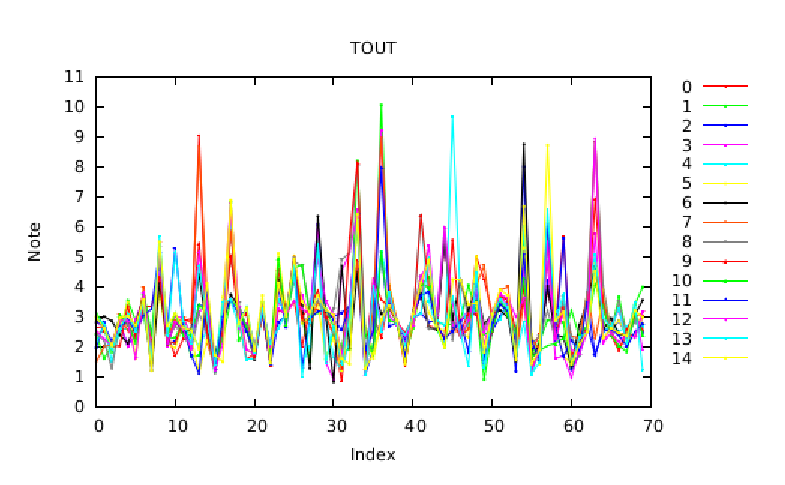
\includegraphics[height=250pt]{images/plot_1.eps}
	\caption{In such a graph, on a given class (abscissa), the distances could be differently distributed. We have to keep in mind this to design a distance.}
	\label{graph}
\end{figure}

% TODO Enlever les légendes?

One example is given in figure \ref{graph}. This set of curve is quite dense, but we can (quite) easily distinguish the possible behaviours of the value.

In some classes, all the images are very similar (for example in the \texttt{apple} class). In the curves, on the right abscissa corresponding to these class (for instance \texttt{apple}), we can see that all the Earth Mover Distances are closed. On the opposite, when there are very different images on the same class (as in the figure \ref{horseshoes}), the EMD values could be very different.

\begin{figure}[!ht]
    \centering
    \subfloat{
        \label{horseshoes:1}
        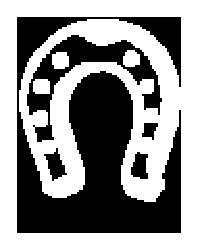
\includegraphics[height=80pt]{images/horseshoe-12}
    }
    \subfloat{
        \label{horseshoes:2}
        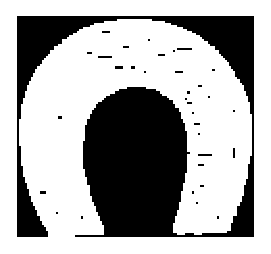
\includegraphics[height=80pt]{images/horseshoe-6}
    }
    \subfloat{
        \label{horseshoes:3}
        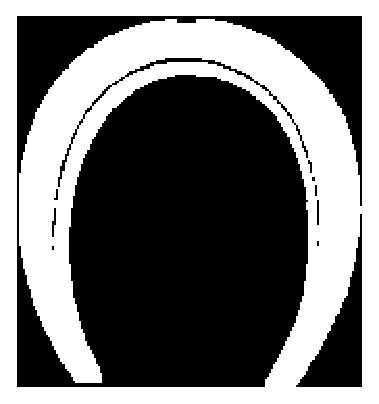
\includegraphics[height=80pt]{images/horseshoe-4}
    }
	\subfloat{
        \label{horseshoes:4}
        
\includegraphics[height=80pt]{images/horseshoe-2}
    }
    \caption{In a single class (here \texttt{horseshoe}), we can have images with different granulometric functions, and so different EMDs to a same image} 
	\label{horseshoes}
\end{figure}

Hence, on such graphs, we can see the two different behaviours: 
\begin{itemize}
	\item All the distances can be closed but not to 0;
	\item The distances are quite distributed.
\end{itemize}

\subsubsection{Definition of the distance}

The goal of the previous analysis was to decide what importance to give to low and high Earth Mover Distances.

For example, take the mean of the distance would be a bad solution, since we can have an image very close to the input but all the other one in the class give important distances.

On the curves, we also observe that the minimum of all the distance gives quite good results (i.e on the first five choices overall). These are all the reasons that why we use this distance:

\begin{definition}
	Let $\mathcal{C} = \set{c_1,\dots,c_n}$ be a class of $n$ histograms (images), and $c$ be an histogram of an image $\mathcal{X}$. We define the distance between the image and the class by the quantity:

\[
	Dist(\mathcal{X},\mathcal{C}) = \underset{i = 1 \dots n}{\operatorname{min}} \left( EMD(c_i,c) \right)
\]

\end{definition}

Let's now test our shape retrieval system.

\subsubsection{Experiments}

For the experiments, we run the script given to evaluate our shape indexing algorithm. It builds a perturbed image (rotation, scaling and adding specular noise) from a random image of the database, and then runs our algorithm to get the rank of the correct class. If the rank belongs to $\set{1,\dots,10}$, the algorithm succeeds.

%TODO Details about the experiment

\begin{table}[h!]
  \centering
  \begin{tabular}{ | m{2.2cm} | m{2.2cm} | m{2.2cm} | m{2.2cm} | m{2.2cm} | m{2.2cm} | }
    \hline
    original & first & second & third & fourth & fifth \\
	\hline
	% Experience 1
    \begin{minipage}{.3\textwidth}
      
\includegraphics[width=\linewidth, width=20mm]{images/test-apple}
    \end{minipage}
    &
    \begin{minipage}{.3\textwidth}
      
\includegraphics[width=\linewidth, width=20mm]{images/apple-1}
    \end{minipage}
    & 
    \begin{minipage}{.3\textwidth}
      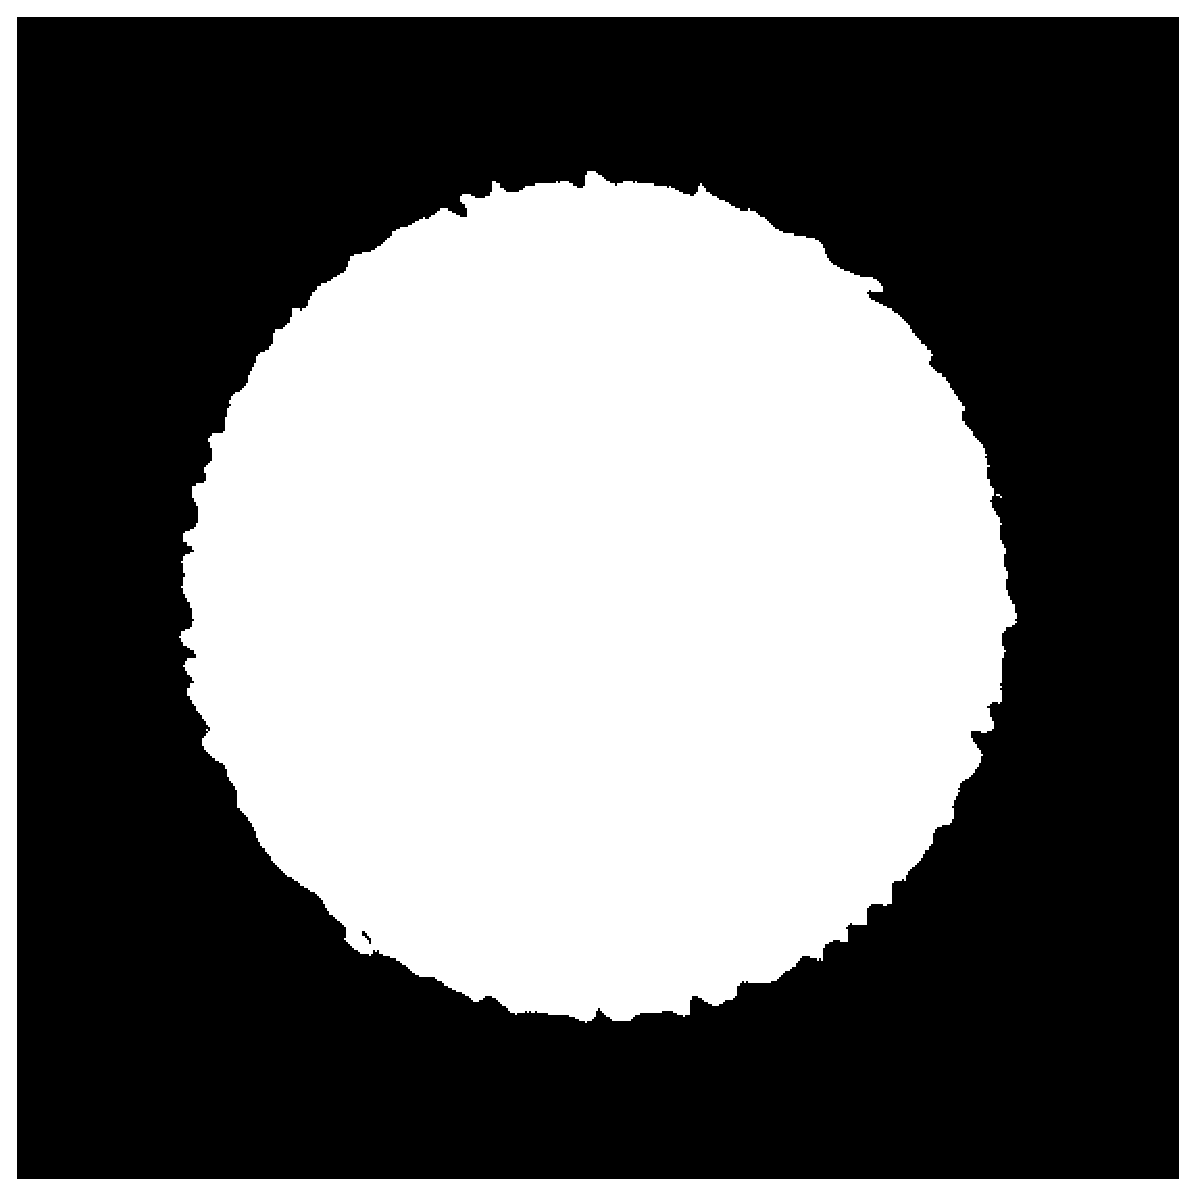
\includegraphics[width=\linewidth, width=20mm]{images/device9}
    \end{minipage}
	&
	\begin{minipage}{.3\textwidth}
      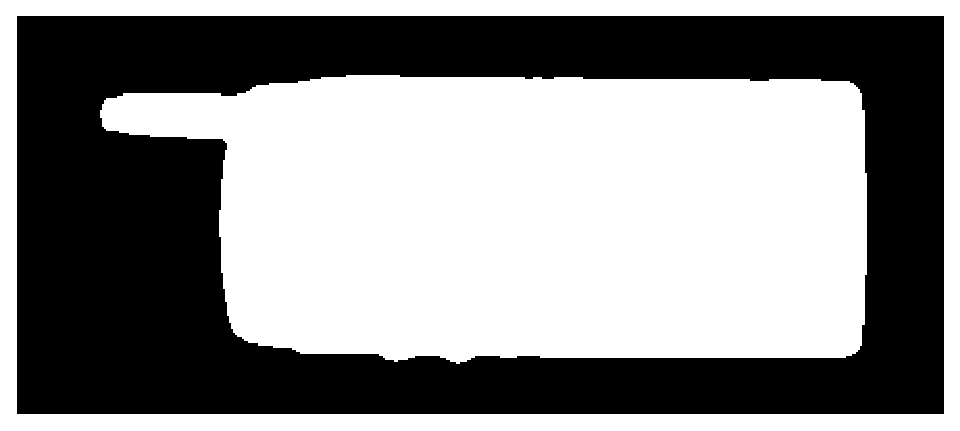
\includegraphics[width=\linewidth, width=20mm]{images/cellular_phone}
    \end{minipage}
	&
    \begin{minipage}{.3\textwidth}
      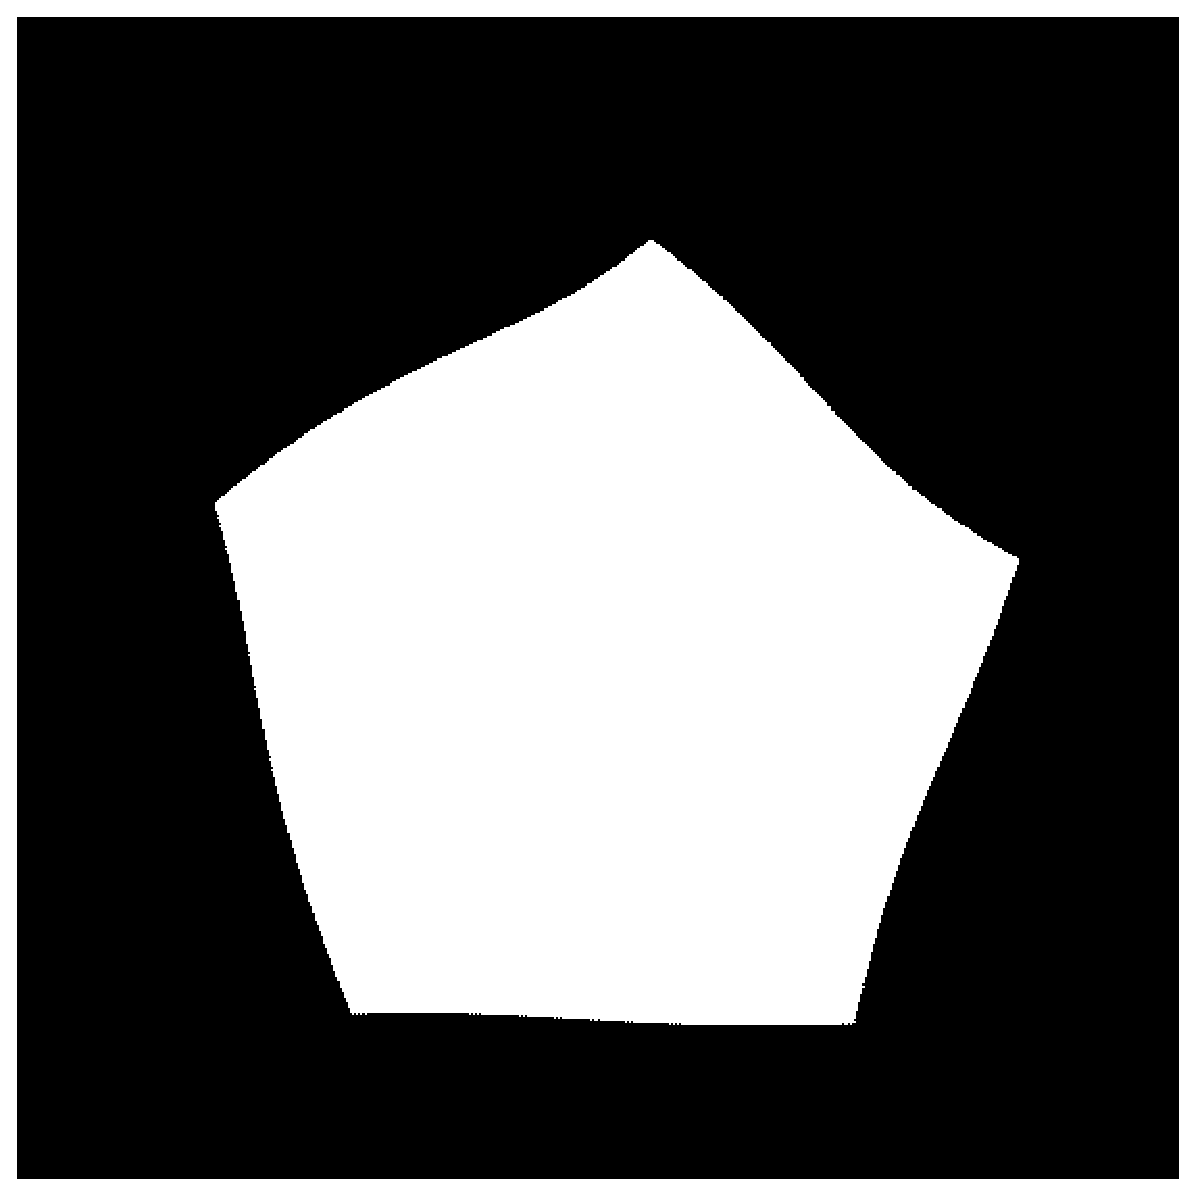
\includegraphics[width=\linewidth, width=20mm]{images/device6}
    \end{minipage}
	&
    \begin{minipage}{.3\textwidth}
      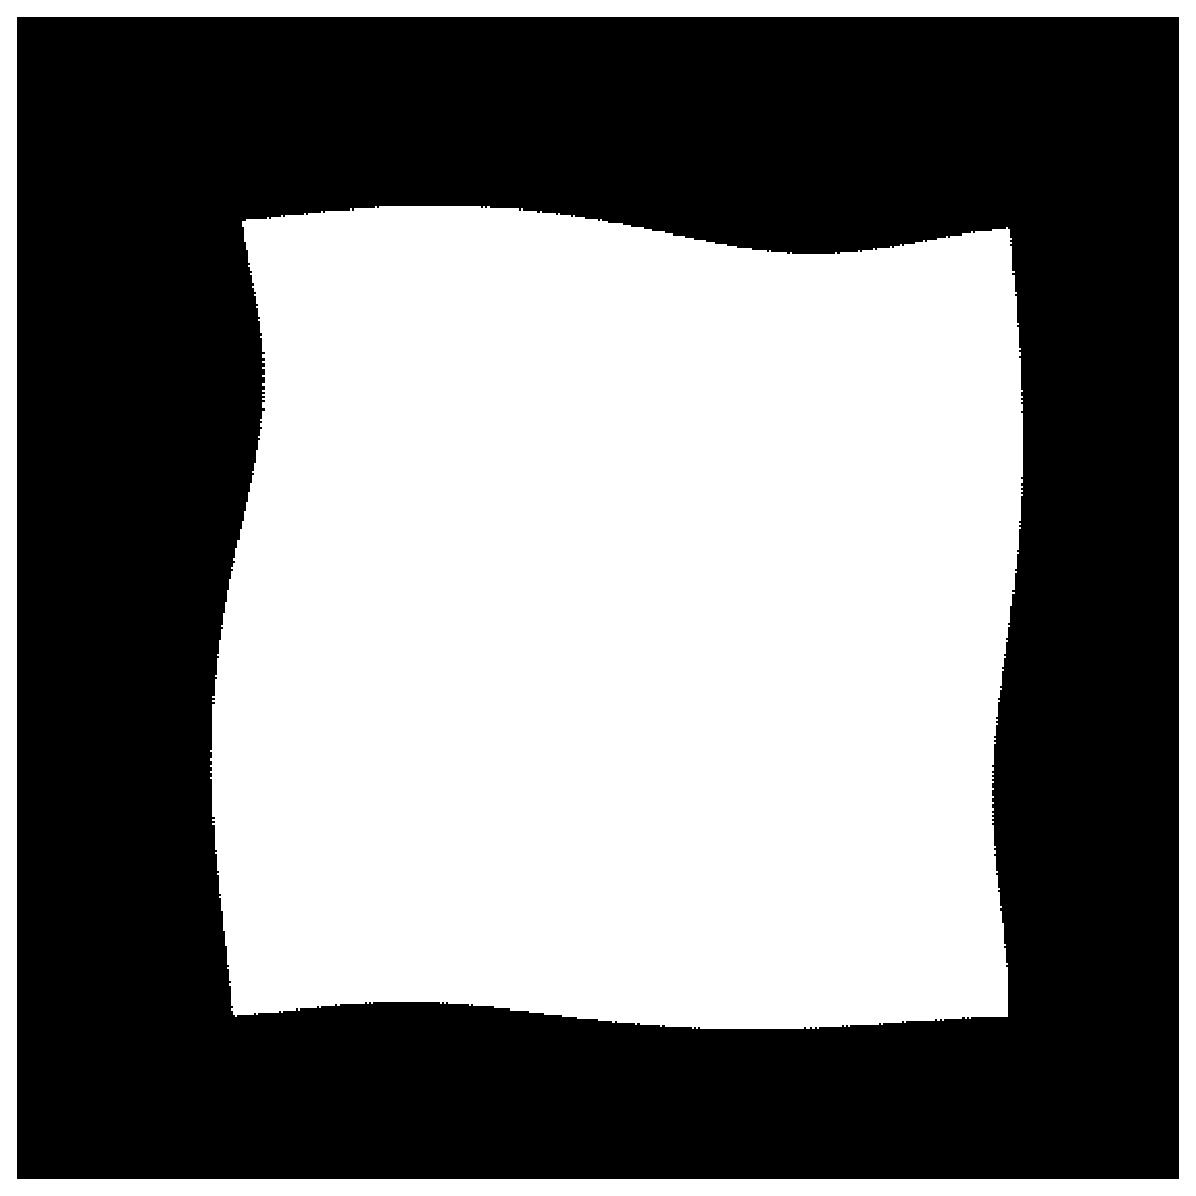
\includegraphics[width=\linewidth, width=20mm]{images/device3}
    \end{minipage}
	\\ \hline
	apple & apple & device9 & cellular\_phone & device6 & device3 \\ \hline
	score & 0.984914 & 0.964994 & 0.949397 & 0.929609 & 0.924559 \\ \hline
	% Experience 2
	\begin{minipage}{.3\textwidth}
      
\includegraphics[width=\linewidth, width=20mm]{images/test-bone}
    \end{minipage}
    &
    \begin{minipage}{.3\textwidth}
      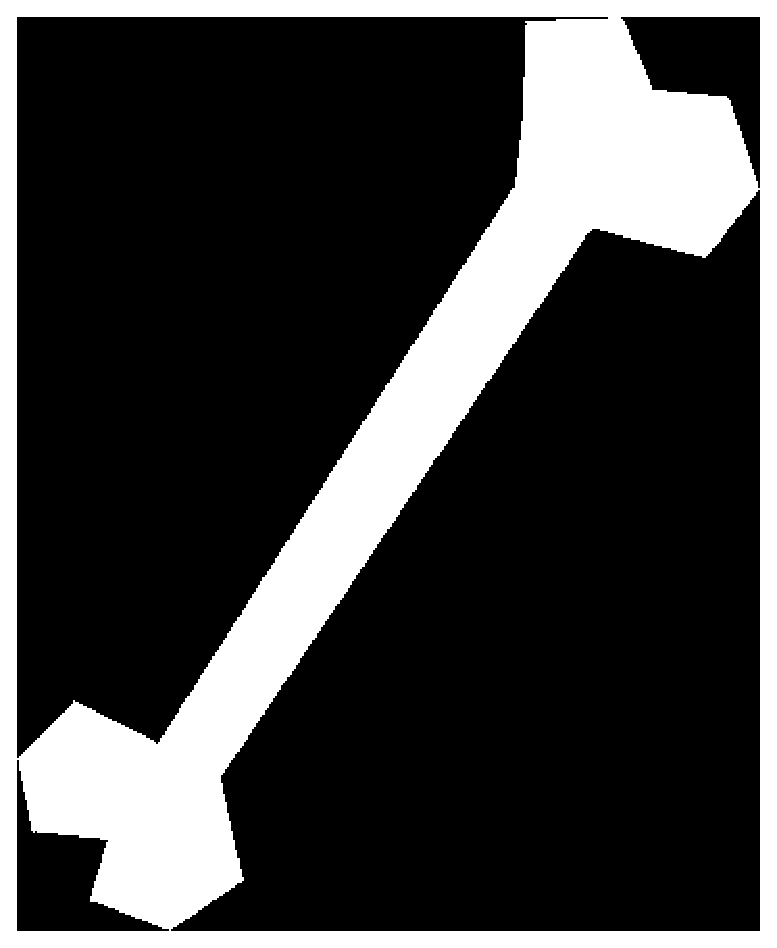
\includegraphics[width=\linewidth, width=20mm]{images/bone}
    \end{minipage}
    & 
    \begin{minipage}{.3\textwidth}
      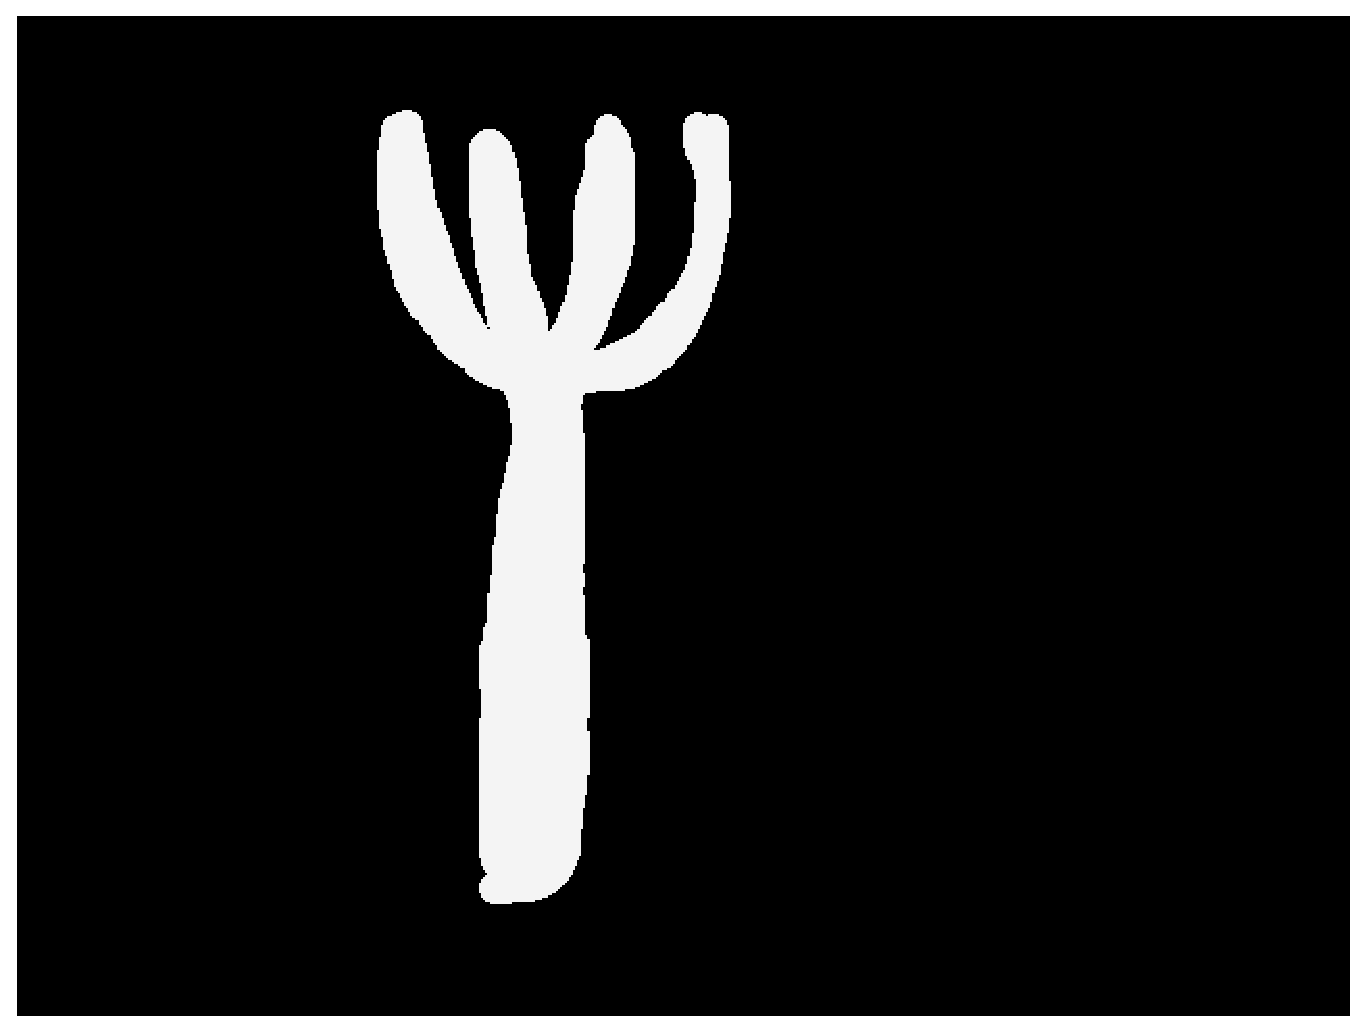
\includegraphics[width=\linewidth, width=20mm]{images/fork}
    \end{minipage}
	&
	\begin{minipage}{.3\textwidth}
      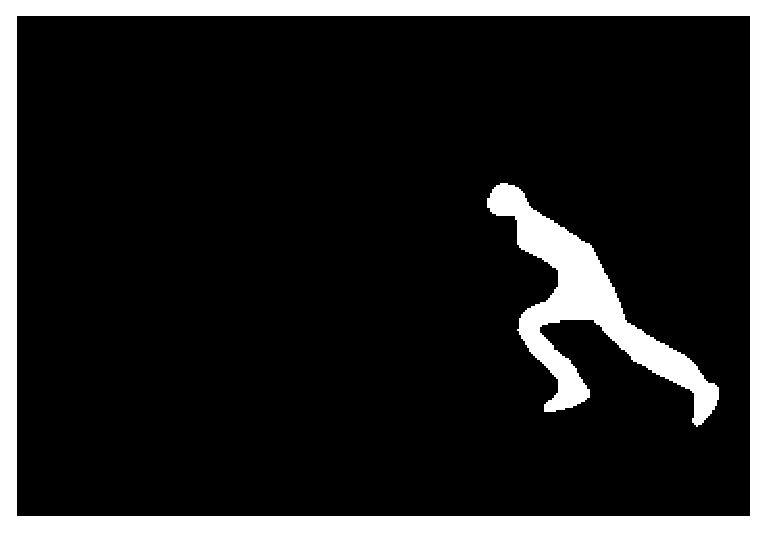
\includegraphics[width=\linewidth, width=20mm]{images/stef}
    \end{minipage}
	&
    \begin{minipage}{.3\textwidth}
      
\includegraphics[width=\linewidth, width=20mm]{images/device8}
    \end{minipage}
	&
    \begin{minipage}{.3\textwidth}
      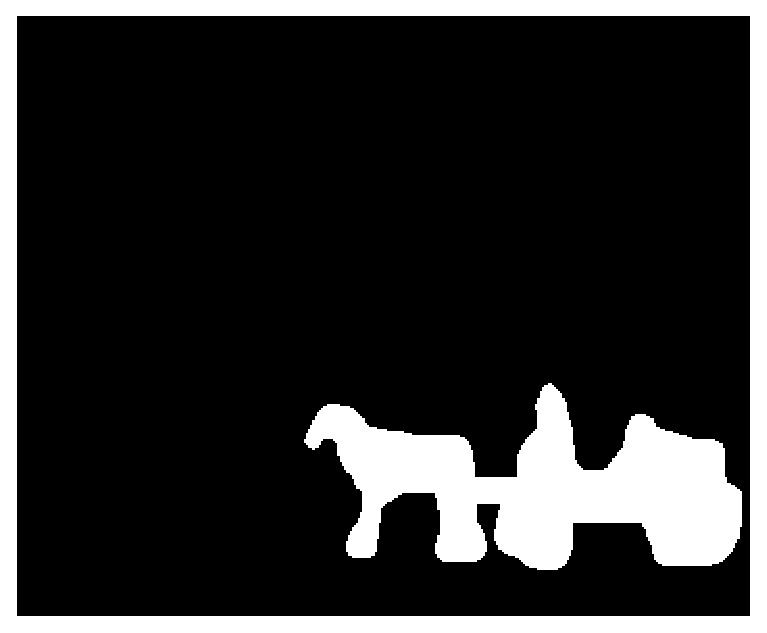
\includegraphics[width=\linewidth, width=20mm]{images/carriage}
    \end{minipage}
	\\ \hline
	bone & bone & fork & stef & device8 & carriage \\ \hline
	score & 0.945207 & 0.883185 & 0.873859 & 0.86771 & 0.844169 \\ \hline
  \end{tabular}
  \caption{Our results of retrieval run on the right side image. For some images, the classes found could be surprising, but there are a larger gap between the better mark and the furthers.}
\end{table}

% Note, on voit les images sous une faible résolution, en réalité les images sont plus grandes et le bruit est bien plus perceptible
% --> Mentionner cela.

\section*{Conclusion}

The goal of this project was not to implement the maximal number of image indexing processes and to mix them on a single tool with any coherence and fancy linear combination. Our approach was to start with a fixed first idea, the granulometric function, and to work around it in order to see the benefits and disadvantages of methods based on it. We saw that with the granulometric function we can give a representation of the object in terms of thickness, which models the concept of segmentation we use implicitly to recognize objects. We used different algorithms to compute it and proved their correctness. With our experiments, we checked the expected performances. Therefore, one could improve this shape retrieval system, mostly by speed up the granulometric computations, which take too much time to be used in practice. Another possible improvement could be to search how to integrate the spatial information lost in the granulometric function.


\bibliographystyle{plain}
\bibliography{biblio}

\end{document}

